\documentclass[12pt]{book}
\usepackage[utf8]{inputenc}
\usepackage[T1,T2A]{fontenc}
\usepackage{graphicx}
\usepackage{setspace}
\usepackage{enumitem}
\setstretch{1.0} % line spacing
%\setlength{\parskip}{0.1cm} % spacing between paragraphs
\usepackage{geometry}
\usepackage{caption}
%\captionsetup[table]{name=\textsc{Таблица}}
%\captionsetup[table]{justification=raggedleft, singlelinecheck=off}
\usepackage[labelsep=period]{caption}
\geometry{a4paper, portrait, left=30mm, right=15mm, top=20mm, bottom=20mm, bindingoffset=0mm}
\usepackage[english,russian]{babel}
% \renewcommand{\chaptername}{Глава}
\usepackage[export]{adjustbox}
\usepackage{xcolor}
\usepackage{titlesec}
\titleformat{\chapter}[block]{\large\bfseries\filcenter}{\thechapter.\hspace{-4mm}}{1em}{}
\titleformat{\section}[block]{\large\bfseries\filcenter}{\thesection.\hspace{-4mm}}{1em}{}
\titleformat{\subsection}[block]{\large\bfseries\filcenter}{\thesubsection.\hspace{-4mm}}{1em}{}
\titlespacing*{\chapter}{0pt}{0.0ex}{3.0ex}
\usepackage{indentfirst}
\usepackage{fancyhdr}
\fancyhf{}
\fancyfoot[C]{\large\thepage}
\renewcommand{\headrulewidth}{0pt}
\pagestyle{fancy}
\clearpage
\setcounter{page}{8} % number of start page
\setcounter{chapter}{1} % chapter number minus one
\setlength{\footnotesep}{0.5cm} % the space between footnotes
\setlength{\skip\footins}{0.5cm} % the space between the text body and the footnotes

% Starting chapters on even-numbered pages
\makeatletter
\renewcommand*\cleardoublepage{\clearpage\if@twoside
  \ifodd\c@page \hbox{}\newpage\if@twocolumn\hbox{}%
  \newpage\fi\fi\fi}
\makeatother

\usepackage{afterpage}
\newcommand\myemptypage{
    \null
    %\thispagestyle{empty}
    \addtocounter{page}{-1}
    \newpage
    }

\usepackage{cite} % Работа с библиографией
%\usepackage[superscript]{cite} % Ссылки в верхних индексах
%\usepackage[nocompress]{cite} % 
\usepackage{csquotes} % Еще инструменты для ссылок

\usepackage{blindtext}%
\usepackage{etoolbox}%

\patchcmd{\thebibliography}{\chapter*}{\par\let\clearpage\relax\chapter*}{\typeout{success}}{\typeout{failure}}


\begin{document}

%\myemptypage

\chapter*{\textsc{Глава 1. Введение в голосовую биометрию}}

%\thispagestyle{empty}
\thispagestyle{fancy}

\large{Настоящая глава является вводной и посвящена рассмотрению общих вопросов, связанных с биометрией, в том числе голосовой. Материал главы затрагивает причины использования биометрических систем, биометрические признаки, устройство биометрической системы и ошибки, возникающие в ней, вопросы мультимодальной биометрии, основные определения и решаемые задачи в области голосовой биометрии, конвейер голосовой биометрии, критерии надёжности систем голосовой биометрии, основные сложности при решении задач голосовой биометрии, примеры практического использования систем голосовой биометрии, биометрические стандарты, текущее состояние дел, нерешённые проблемы и~перспективные направления в области голосовой биометрии.}

\section{Зачем нужны биометрические системы?}

\large{В современном мире увеличение числа преступлений, грабежей и вооружённых нападений ставит ряд вопросов перед разработчиками существующих систем безопасности: \textit{«Насколько эффективны существующие системы безопасности?»}, \textit{«Гарантируют ли эти системы требуемый уровень безопасности?»}, \textit{«Способны ли эти системы надёжно определять неавторизованного пользователя?»}, \textit{«Удобно ли пользоваться этими системами?»}. На ранних этапах развития систем определения личности активно использовались криптографические методы, требующие от пользователя знания пароля или, например, наличия карты для подтверждения личности. Поэтому окружающий нас мир наводнён паролями и картами, необходимыми для получения доступа к определённым ресурсам: информация на персональном компьютере или мобильном устройстве, электронная почта, банковские счета и т.п. У пользователей подобных систем возникает множество вопросов:  \textit{«Что случится, если будет забыт пароль или утеряна карта?»}, \textit{«Какие потери, например, в деньгах возникнут, если пароль узнает злоумышленник?»}, \textit{«Насколько много паролей требуется помнить?»}, \textit{«Насколько много карт требуется хранить?»}, \textit{«Как система определяет, кто запрашивает доступ к некоторым ресурсам?»}, \textit{«Есть ли альтернатива удобнее и надёжнее?»}. В качестве ответа на поставленные вопросы научное сообщество предлагает воспользоваться идеей распознавания личности на основе физиологических и поведенческих признаков/характеристик/атрибутов/модальностей. Данное распознавание относят к~термину \textit{биометрия} (от др.-греч. $\beta \iota o \zeta$ -- жизнь и $\mu \varepsilon \tau \varrho \varepsilon \omega$ -- измеряю).}

\large{В области информатики биометрия рассматривается в качестве набора инструментов, предназначенных для автоматизированного или автоматического\footnote{Термин «автоматизированный», в отличие от термина «автоматический», подчёркивает сохранение за человеком-оператором некоторых функций, либо наиболее общего, целеполагающего характера, либо не поддающихся реализации в автоматическом режиме.} распознавания личности по её уникальным физиологическим (отпечаток пальца, изображение лица, радужная оболочка и т.п.) и поведенческим атрибутам (голос, походка, подпись и т.п.). Необходимо отметить, что использование биометрических инструментов на практике не является идеальным решением, однако предоставляет ряд преимуществ перед знанием пароля или наличием карты у пользователя: 

\begin{itemize}[topsep=1pt] \itemsep0.1em
\item «не нужно ничего запоминать»;
\item биометрические атрибуты сложнее потерять, передать или украсть;
\item обеспечение лучшей безопасности, из-за того, что биометрические атрибуты сложно подделать и требуется присутствие настоящего пользователя при предоставлении доступа к определённым ресурсам.
\end{itemize}

Вдохновленное разработкой первой биометрической системы Альфонсом Бертильоном\footnote{Система бертильонаж (от фр. bertillonnage) -- первая система идентификации преступников по их антропометрическим данным (длина ступней, длина рук и т.п.), разработанная французским юристом и изобретателем Альфонсом Бертильоном в 1883 г.} в 1883 г. и элементарной системой распознавания отпечатков пальцев сэром Джоном Гальтоном\footnote{Первый метод классификации отпечатков пальцев был разработан в 1892 г. сэром Джоном Гальтоном. В качестве основных признаков для идентификации в методе рассматривались минуции, т.е. участки папиллярного рисунка кожи, где отдельные линии сливаются, раздваиваются или обрываются.} в 1892 г. научное сообщество направило свои усилия на изучение различных биометрических модальностей. Любые физиологические и поведенческие атрибуты могут рассматриваться в качестве биометрических признаков, если они удовлетворяют следующим критериям: 

\begin{itemize}[topsep=1pt] \itemsep0.1em
\item \textit{универсальность} (любая личность способна предоставить требуемый биометрический образец);
\item \textit{дискриминативность} (биометрические признаки разных личностей должны различаться);
\item \textit{инвариантность} (неизменность биометрических атрибутов с течением времени);
\item \textit{собираемость} (простота накопления биометрических атрибутов в процессе их захвата определённым оборудованием, оцифровки и извлечения признаков);
\item \textit{эффективность} (возможность получения высоких показателей качества работы системы для выбранных биометрических признаков);
\item \textit{приемлемость} (готовность личности предоставить требуемый биометрический образец);
\item \textit{защищённость} (сложность подделки биометрических атрибутов в случае мошеннических/спуфинг атак на систему).
\end{itemize}

}

\section{Биометрические признаки}

\large{Биометрические признаки -- это четкие, индивидуальные, биологически обусловленные характеристики каждого человека. Применительно к критериям, представленным выше, можно ввести следующую классификацию биометрических признаков:

\begin{itemize}[topsep=1pt] \itemsep0.1em
\item \textit{физиологические признаки} -- атрибуты, относящиеся к физиологии человека. Для удобства физиологические признаки могут быть разделены на подкатегории, соответствующие области расположения атрибутов на теле человека (область руки, область лица, область глаза). Дополнительно к физиологическим признакам можно отнести медико-химические атрибуты;
\item \textit{поведенческие признаки} -- атрибуты, относящиеся к особенностям поведения человека;
\item \textit{«мягкие» признаки} -- атрибуты, которые не могут быть использованы самостоятельно при распознавании личности, т.к. определяют её неоднозначно, и выступают в качестве дополнительных признаков к~физиологическим и поведенческим.
\end{itemize}

\begin{table}[h]
\centering
\caption{\label{tab:table_1_1}Классификация биометрических признаков}

\begin{tabular}{|cll|}
\hline
\multicolumn{3}{|c|}{Биометрические признаки}                                                                          \\ \hline
\multicolumn{1}{|c|}{Физиологические} & \multicolumn{1}{c|}{Поведенческие} & \multicolumn{1}{c|}{«Мягкие»}             \\ \hline
\multicolumn{1}{|l|}{\begin{tabular}[c]{@{}l@{}}\textit{Область руки:} отпечаток пальца, \\ отпечаток ладони, геометрия руки, \\ вены на руке, отпечаток сгиба пальца\\ \textit{Область лица:} изображение лица, \\ форма уха, зубы, отпечаток языка\\ \textit{Область глаза:} сетчатка, радужная \\ оболочка, сосудистая сеть склеры \\ \textit{Медико-химические признаки:} запах \\ тела, ДНК, звук сердца, \\ электрокардиограмма\end{tabular}} & \multicolumn{1}{l|}{\begin{tabular}[c]{@{}l@{}}Ритм печати текста на \\ клавиатуре, голос, \\ подпись, походка\end{tabular}} & \begin{tabular}[c]{@{}l@{}}Пол, этничность, \\ рост, шрамы, \\ родинки, \\ татуировки\end{tabular} \\ \hline
\end{tabular}
\end{table}

Более подробная детализация того, что собой представляют физиологические, поведенческие и «мягкие» признаки, представлена в табл.~\ref{tab:table_1_1}.}

\subsection{Биометрические признаки в области руки}

\large{Здесь какой-то текст!}

\begin{figure}[h]
\center{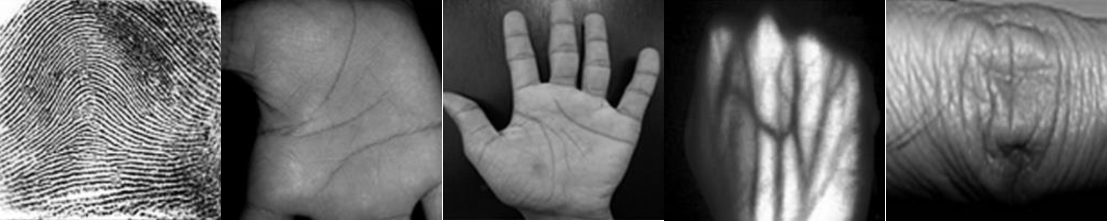
\includegraphics[width=1\linewidth]{images/chapter_01/figure_1_2.pdf}}
\caption{Биометрические признаки в области руки (слева направо): отпечаток пальца, отпечаток ладони, геометрия руки, рисунок вен на руке, отпечаток сгиба пальца}
\label{fig:figure_1_2}
\end{figure}

\subsection{Биометрические признаки в области лица}

\large{Здесь какой-то текст!}

\begin{figure}[h]
\center{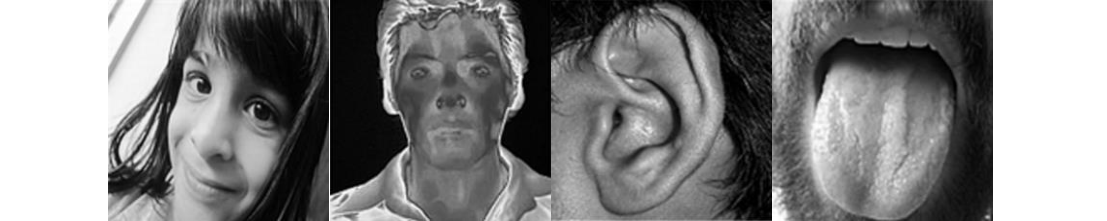
\includegraphics[width=1\linewidth]{images/chapter_01/figure_1_3.pdf}}
\caption{Биометрические признаки в области лица (слева направо): изображение лица, термограмма лица, форма уха, отпечаток языка}
\label{fig:figure_1_3}
\end{figure}

\subsection{Биометрические признаки в области глаза}

\large{Здесь какой-то текст!}

\begin{figure}[h]
\center{
\includegraphics[width=1\linewidth]{images/chapter_01/figure_1_4.pdf}}
\caption{Биометрические признаки в области глаза (слева направо): радужная оболочка, сетчатка, склера и сосудистая сеть}
\label{fig:figure_1_4}
\end{figure}

\subsection{Медико-химическая биометрия}

\large{Здесь какой-то текст!}

\subsection{Поведенческая биометрия}

\large{Здесь какой-то текст!}

\begin{figure}[h]
\center{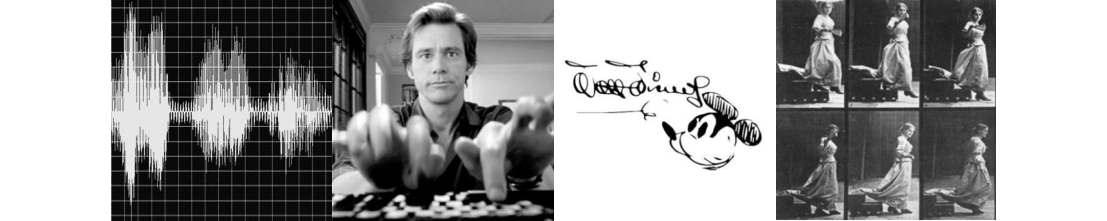
\includegraphics[width=1\linewidth]{images/chapter_01/figure_1_5.pdf}}
\caption{Поведенческая биометрия (слева направо): речевой сигнал, ритм печати текста на клавиатуре, подпись, походка}
\label{fig:figure_1_5}
\end{figure}

\subsection{«Мягкая» биометрия}

\large{Здесь какой-то текст!}

\begin{figure}[h]
\center{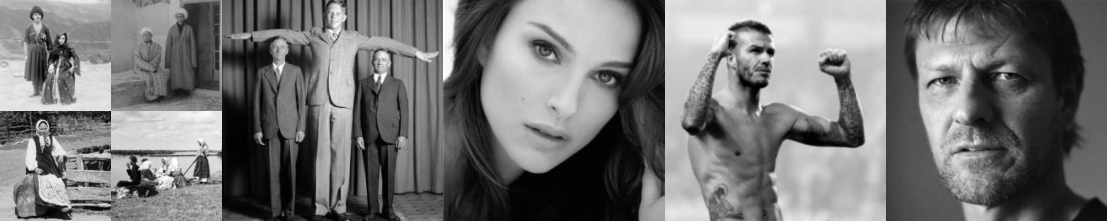
\includegraphics[width=1\linewidth]{images/chapter_01/figure_1_6.pdf}}
\caption{Примерами признаков, используемых в «мягкой» биометрии, являются этничность, рост, родинки, татуировки, шрамы}
\label{fig:figure_1_6}
\end{figure}

\section{Что такое биометрическая система?}

\large{\textit{Биометрическая система} -- это автоматизированная или автоматическая система, решающая две связанные между собой задачи: 

\begin{itemize}[topsep=1pt] \itemsep0.1em
\item \textit{получение биометрических данных} от конечных пользователей с использованием сформированных пользовательских данных (речевые записи, изображения лиц и т.п.);
\item дальнейшее \textit{использование биометрических данных}.
\end{itemize}

\begin{figure}[h]
\center{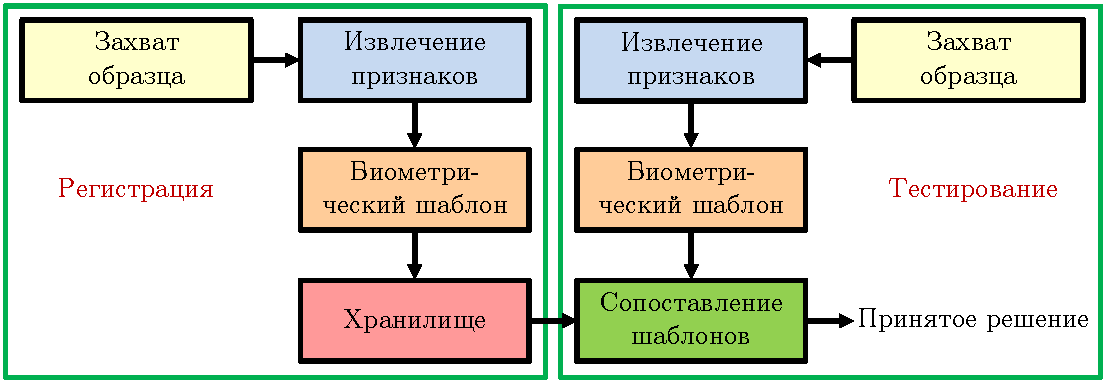
\includegraphics[width=1\linewidth]{images/chapter_01/figure_1_1.pdf}}
\caption{Общая блок-схема биометрической системы: регистрация эталона и сравнение теста с эталоном/эталонами}
\label{fig:figure_1_1}
\end{figure}

К основным \textit{компонентам биометрической системы} можно отнести следующие модули (см. рис.~\ref{fig:figure_1_1}): 

\begin{itemize}[topsep=1pt] \itemsep0.1em
\item \textit{модуль захвата биометрического образца}, предназначенный для формирования «сырых» данных и их передачи с целью дальнейшей обработки;
\item \textit{модуль извлечения признаков}, выполняющий обработку «сырых» данных с целью извлечения из них характерных, отличительных признаков;
\item \textit{модуль генерации биометрического шаблона}, осуществляющий формирование компактного, высокоуровневого представления биометрического образца;
\item \textit{модуль базы данных/хранилище/галерея}, содержащий биометрические шаблоны, вычисленные для эталонных биометрических образцов, сформированных на этапе регистрации пользователя в системе;
\item \textit{модуль сравнения}, позволяющий выполнить сопоставление биометрического шаблона, выделенного для тестового биометрического образца с шаблоном/шаблонами, содержащимися в базе данных, с целью формирования оценки сравнения, на основе которой принимается биометрическое решение.
\end{itemize}

Рис.~\ref{fig:figure_1_1} показывает, что при использовании биометрической системы первоначально происходит регистрация пользователя в системе. Регистрация сопровождается захватом «сырых» данных, извлечением из них характерных признаков, на основе которых может быть сгенерирован эталонный биометрический шаблон, представленный, обычно, в современных практических приложениях в виде высокоуровневого вектора признаков низкой размерности. Указанный вектор сохраняется в хранилище данных, после чего пользователь считается зарегистрированным в системе. Далее на этапе тестирования выполняется процедура захвата тестового образца, для которого вычисляются признаки и биометрический шаблон. Вычисление признаков и биометрического шаблона на этапе тестирования алгоритмически выполняется идентичным образом, что и на этапе регистрации. Полученный тестовый биометрический шаблон сравнивается с~одним или несколькими эталонами, извлечёнными из хранилища. Результатом сопоставления шаблонов является оценка сравнения, на основе которой принимается биометрическое решение.

Рассматривая биометрические системы в целом, можно выделить следующие основные режимы их работы:

\begin{itemize}[topsep=1pt] \itemsep0.1em
\item \textit{верификация} -- режим, при котором пользователь биометрической системы выдает себя за определенную личность. Установление идентичности в данном случае выполняется с помощью оценки схожести между эталонным шаблоном заявленной личности, находящимся в хранилище данных, и предоставленным системе тестовым шаблоном, сформированным в момент взаимодействия пользователя с биометрической системой. Поскольку в результате верификации один эталонный шаблон сопоставляется с одним тестовым шаблоном, подобный режим сравнения определяют как «один к одному». Выходом при этом является ответ «да» или «нет» об аутентичности сравниваемых биометрических шаблонов;

\item \textit{идентификация} -- режим, при котором требуется отнести пользователя биометрической системы к одной из зарегистрированных личностей. При взаимодействии с биометрической системой пользователь не заявляет своё отношение к определённой личности. Поэтому биометрической системе требуется выполнить сравнение предоставленного пользователем тестового биометрического шаблона со всеми эталонными шаблонами зарегистрированных личностей. Подобный режим работы биометрической системы рассматривают в качестве сравнения «один ко многим», а выходом является метка личности, к которой отнесён пользователь биометрической системы.
\end{itemize}

\textit{Производительность и точность работы биометрической системы} зависят от данных, которые подвержены воздействию условий окружающей среды и ограничениям, связанным с технической реализацией системы. В~качестве факторов окружающей среды, воздействующих на биометрическую систему, можно выделить температуру, влажность, освещённость и~т.п. К факторам технической реализации биометрической системы можно отнести следующие: возможность качественного формирования биометрического образца, состав группы пользователей биометрической системы, временной интервал между формированием эталонного и тестового шаблонов, робастность используемых при построении биометрической системы алгоритмов и т.п. Точность работы биометрической системы обычно описывается в терминах ошибок, связанных с формированием биометрического образца и реализационными ограничениями самой системы:

\begin{itemize}[topsep=1pt] \itemsep0.1em
\item \textit{ошибки при формировании биометрического образца} связывают с условиями окружающей среды, в которых эксплуатируется биометрическая система, и качеством сенсора, используемого для захвата биометрического образца. В~качестве примеров подобного рода ошибок можно выделить, во-первых, процент отклонения биометрической системой захваченного образца, из-за его низкого качества и, во-вторых, неспособность сенсора сформировать валидный биометрический образец;

\item \textit{ошибки реализационных ограничений системы} используются для оценки точности работы биометрической системы в «полевых» условиях. В~качестве примеров подобного рода ошибок можно выделить \textit{долю ложных отрицательных решений} (англ. false reject rate, FRR, или false negative rate, FNR), также называемую \textit{вероятностью ошибки первого рода}, \textit{долю ложных  положительных решений} (англ. false acceptance rate, FAR или false positive rate, FPR), также называемую \textit{вероятностью ошибки второго рода} и \textit{равный уровень ошибок} (англ. equal error rate, EER). \textit{Доля ложных отрицательных решений} описывает долю событий (в~процентах), когда зарегистрированный в системе пользователь отклонён системой на этапе тестирования. С точки зрения удобства взаимодействия пользователя с системой доля ложных отрицательных решений должна быть меньше настолько, насколько возможно. \textit{Доля ложных положительных решений} описывает долю событий (в~процентах), когда незарегистрированный в системе пользователь не отклонён системой на этапе тестирования. Для робастных биометрических систем доля ложных положительных решений должна быть меньше настолько, насколько возможно. Термин \textit{равного уровня ошибок} относят к такой рабочей точке биометрической системы, для которой доля ложных отрицательных решений и доля ложных положительных решений равны между собой.

\end{itemize}

Вероятно, можно считать, что значимость ошибок, возникающих при формировании биометрического образца, является более важной, чем ошибок, связанных с реализационными ограничениями системы, потому что отсутствие возможности формирования качественных данных, используемых для принятия биометрического решения, драматически влияет на ухудшение качества работы биометрической системы в целом. Например, зачастую гораздо проще повысить качество работы биометрической системы через использование более совершенного сенсора для формирования биометрического образца, чем усложнять алгоритмически конвейер обработки некачественно захваченных данных.

}

\section{Мультимодальная биометрия}

\large{Здесь какой-то текст!}

\section{Голосовая биометрическая система}

\large{Здесь какой-то текст!}

\section{Основные задачи, решаемые голосовой биометрической~системой}

\large{Здесь какой-то текст!}

\section{Конвейер голосовой биометрии}

\large{Здесь какой-то текст!}

\section{Критерии надёжности систем голосовой биометрии}

\large{Здесь какой-то текст!}

\section{Примеры практического использования систем голосовой~биометрии}

\large{Здесь какой-то текст!}

\section{Биометрические стандарты}

\large{Здесь какой-то текст!}

\section{Почему распознавание диктора -- сложная задача?}

\large{Здесь какой-то текст!}

\section{Текущее состояние дел в области голосовой биометрии}

\large{Здесь какой-то текст!}

\section{Нерешённые проблемы и перспективные направления в~области голосовой биометрии}

\large{Здесь какой-то текст!

\section*{Контрольные вопросы}

\large{

\begin{enumerate}
\item Что такое биометрия?
\item В чём состоят основные преимущества биометрии перед знанием пароля и использованием карты?
\item Каким основным критериям должны удовлетворять биометрические признаки?
\item Как можно классифицировать биометрические признаки?
\item Что такое биометрическая система?
\item Из каких основных модулей состоит биометрическая система?
\end{enumerate}

}

%\bibliographystyle{IEEEtran}
%\bibliography{mybib}

\cite{Bardhan,Fama2,qwerty}

\renewcommand{\bibname}{Список литературы}

\begin{thebibliography}{9}
    \thispagestyle{fancy}
    \addcontentsline{toc}{section}{\bibname}
    \bibitem{qwerty} Источник номер 1
    \bibitem[Fama, 1965]{Fama} Fama E. F. The behavior of stock-market prices //Journal of business. – 1965. – С. 34-105.
    \bibitem{Fama2} Fama E. F. Random walks in stock market prices //Financial Analysts Journal. – 1965. – С. 55-59.
    \bibitem{Bardhan} Bardhan P. Corruption and development: a review of issues //Journal of Economic Literature. 1997. 35.3, с. 1320—1346.
\end{thebibliography}

\end{document}
